\documentclass{report}
\usepackage{graphicx, tikz-cd, float, titlepic, booktabs} % Required for inserting images
\usepackage{pgfplots}
\pgfplotsset{compat=1.15}
\usepackage{mathrsfs}
\usetikzlibrary{arrows}
\usepackage{amsmath, amssymb, amsthm, amsfonts, siunitx, physics, gensymb}
\AtBeginDocument{\RenewCommandCopy\qty\SI}
\usepackage[version=4]{mhchem}
\usepackage[most,many,breakable]{tcolorbox}
\usepackage{xcolor, fancyhdr, varwidth}
\usepackage[Glenn]{fncychap}
%Options: Sonny, Lenny, Glenn, Conny, Rejne, Bjarne, Bjornstrup
\usepackage{hyperref, cleveref}
\usepackage{icomma, enumitem} %comma as decimal and continue enumerate with [resume]
\usepackage[danish]{babel}
%%%%%%%%%%%%%%%%%%%%%%%%%%%%%%
% SELF MADE COLORS
%%%%%%%%%%%%%%%%%%%%%%%%%%%%%%
\definecolor{myg}{RGB}{56, 140, 70}
\definecolor{myb}{RGB}{45, 111, 177}
\definecolor{myr}{RGB}{199, 68, 64}
\definecolor{mytheorembg}{HTML}{F2F2F9}
\definecolor{mytheoremfr}{HTML}{00007B}
\definecolor{mylenmabg}{HTML}{FFFAF8}
\definecolor{mylenmafr}{HTML}{983b0f}
\definecolor{mypropbg}{HTML}{f2fbfc}
\definecolor{mypropfr}{HTML}{191971}
\definecolor{myexamplebg}{HTML}{F2FBF8}
\definecolor{myexamplefr}{HTML}{88D6D1}
\definecolor{myexampleti}{HTML}{2A7F7F}
\definecolor{mydefinitbg}{HTML}{E5E5FF}
\definecolor{mydefinitfr}{HTML}{3F3FA3}
\definecolor{notesgreen}{RGB}{0,162,0}
\definecolor{myp}{RGB}{197, 92, 212}
\definecolor{mygr}{HTML}{2C3338}
\definecolor{myred}{RGB}{127,0,0}
\definecolor{myyellow}{RGB}{169,121,69}
\definecolor{myexercisebg}{HTML}{F2FBF8}
\definecolor{myexercisefg}{HTML}{88D6D1}
%%%%%%%%%%%%%%%%%%%%%%%%%%%%%%%%%%%%%%%%%%%%%%%%%%%%%%%%%%%%%%%%%%%%%%
% Box environments for theorems and problems
%%%%%%%%%%%%%%%%%%%%%%%%%%%%%%%%%%%%%%%%%%%%%%%%%%%%%%%%%%%%%%%%%%%%%
\setlength{\parindent}{1cm}
%================================
% Question BOX
%================================
\makeatletter
\newtcbtheorem{question}{Opgave}{enhanced,
	breakable,
	colback=white,
	colframe=myb!80!black,
	attach boxed title to top left={yshift*=-\tcboxedtitleheight},
	fonttitle=\bfseries,
	title={#2},
	boxed title size=title,
	boxed title style={%
			sharp corners,
			rounded corners=northwest,
			colback=tcbcolframe,
			boxrule=0pt,
		},
	underlay boxed title={%
			\path[fill=tcbcolframe] (title.south west)--(title.south east)
			to[out=0, in=180] ([xshift=5mm]title.east)--
			(title.center-|frame.east)
			[rounded corners=\kvtcb@arc] |-
			(frame.north) -| cycle;
		},
	#1
}{def}
\makeatother
%================================
% DEFINITION BOX
%================================

\newtcbtheorem[]{Definition}{Definition}{enhanced,
	before skip=2mm,after skip=2mm, colback=red!5,colframe=red!80!black,boxrule=0.5mm,
	attach boxed title to top left={xshift=1cm,yshift*=1mm-\tcboxedtitleheight}, varwidth boxed title*=-3cm,
	boxed title style={frame code={
					\path[fill=tcbcolback]
					([yshift=-1mm,xshift=-1mm]frame.north west)
					arc[start angle=0,end angle=180,radius=1mm]
					([yshift=-1mm,xshift=1mm]frame.north east)
					arc[start angle=180,end angle=0,radius=1mm];
					\path[left color=tcbcolback!60!black,right color=tcbcolback!60!black,
						middle color=tcbcolback!80!black]
					([xshift=-2mm]frame.north west) -- ([xshift=2mm]frame.north east)
					[rounded corners=1mm]-- ([xshift=1mm,yshift=-1mm]frame.north east)
					-- (frame.south east) -- (frame.south west)
					-- ([xshift=-1mm,yshift=-1mm]frame.north west)
					[sharp corners]-- cycle;
				},interior engine=empty,
		},
	fonttitle=\bfseries,
	title={#2},#1}{def}
\newtcbtheorem[]{definition}{Definition}{enhanced,
	before skip=2mm,after skip=2mm, colback=red!5,colframe=red!80!black,boxrule=0.5mm,
	attach boxed title to top left={xshift=1cm,yshift*=1mm-\tcboxedtitleheight}, varwidth boxed title*=-3cm,
	boxed title style={frame code={
					\path[fill=tcbcolback]
					([yshift=-1mm,xshift=-1mm]frame.north west)
					arc[start angle=0,end angle=180,radius=1mm]
					([yshift=-1mm,xshift=1mm]frame.north east)
					arc[start angle=180,end angle=0,radius=1mm];
					\path[left color=tcbcolback!60!black,right color=tcbcolback!60!black,
						middle color=tcbcolback!80!black]
					([xshift=-2mm]frame.north west) -- ([xshift=2mm]frame.north east)
					[rounded corners=1mm]-- ([xshift=1mm,yshift=-1mm]frame.north east)
					-- (frame.south east) -- (frame.south west)
					-- ([xshift=-1mm,yshift=-1mm]frame.north west)
					[sharp corners]-- cycle;
				},interior engine=empty,
		},
	fonttitle=\bfseries,
	title={#2},#1}{def}

\newtcbtheorem{theo}%
    {Theorem}{}{theorem}
\newtcolorbox{prob}[1]{colback=red!5!white,colframe=red!50!black,fonttitle=\bfseries,title={#1}}
%================================
% NOTE BOX
%================================

\usetikzlibrary{arrows,calc,shadows.blur}
\tcbuselibrary{skins}
\newtcolorbox{note}[1][]{%
	enhanced jigsaw,
	colback=gray!20!white,%
	colframe=gray!80!black,
	size=small,
	boxrule=1pt,
	title=\textbf{Note:},
	halign title=flush center,
	coltitle=black,
	breakable,
	drop shadow=black!50!white,
	attach boxed title to top left={xshift=1cm,yshift=-\tcboxedtitleheight/2,yshifttext=-\tcboxedtitleheight/2},
	minipage boxed title=1.5cm,
	boxed title style={%
			colback=white,
			size=fbox,
			boxrule=1pt,
			boxsep=2pt,
			underlay={%
					\coordinate (dotA) at ($(interior.west) + (-0.5pt,0)$);
					\coordinate (dotB) at ($(interior.east) + (0.5pt,0)$);
					\begin{scope}
						\clip (interior.north west) rectangle ([xshift=3ex]interior.east);
						\filldraw [white, blur shadow={shadow opacity=60, shadow yshift=-.75ex}, rounded corners=2pt] (interior.north west) rectangle (interior.south east);
					\end{scope}
					\begin{scope}[gray!80!black]
						\fill (dotA) circle (2pt);
						\fill (dotB) circle (2pt);
					\end{scope}
				},
		},
	#1,
}

%%%%%%%%%%%%%%%%%%%%%%%%%%%%%%%%%%%%%%%%%%%%%%%%%%%%%%%%%%%%%%%%%
% SELF MADE COMMANDS
%%%%%%%%%%%%%%%%%%%%%%%%%%%%%%
\newcommand{\sol}{\setlength{\parindent}{0cm}\textbf{\textit{Løsning:}}\setlength{\parindent}{1cm}}
%%%%%%%%%%%%%%%%%%%%%%%%%%%%%%%%%
\usepackage[tmargin=2cm,rmargin=1in,lmargin=1in,margin=0.85in,bmargin=2cm,footskip=.2in]{geometry}\pagestyle{fancy}
\lhead{Minrui Kevin Zhou 2.b}
\rhead{Opgavesæt 4}

\title{Opgavesæt 4\\
{\Large \textbf{2.b kemi A}}}
\author{Kevin Zhou}
\date{\today}

\begin{document}
\maketitle
\begin{note}
  Alle værdier ikke givet af opgavebogen er taget fra databogen
\end{note}
\section*{Opgave 2.18 A}
\sol \\
\textbf{a.} 
Vi beregner først massen af chlor.
\begin{equation*}
\begin{split}
  m(\text{\ce{Cl}} )&=m(\text{stof} )-m(\ce{C} )-m(\ce{H} )\\ 
  &=1,486 \;\unit{g} -0,368 \;\unit{g} -0,031 \;\unit{g} \\ 
  &=1,087 \;\unit{g} 
\end{split}
\end{equation*}
Vi kan da nu regne stofmængderne af \ce{C}, \ce{H} og \ce{Cl}:
\begin{equation*}
\begin{split}
  &n(\ce{C} )=\frac{0,368 \;\unit{g} }{12,01 \;\unit{g/mol} }=30,6411 \;\unit{mmol} \\ 
  &n(\ce{H} )=\frac{0,031 \;\unit{g} }{1,008 \;\unit{g/mol} }=30,7540 \;\unit{mmol} \\ 
  &n(\ce{Cl} )=\frac{1,087 \;\unit{g} }{35,45 \;\unit{g/mol} }=30,6629 \;\unit{mmol} 
\end{split}
\end{equation*}
Vi ser da, at
\begin{equation*}
\begin{split}
  \frac{n(\ce{C} )}{n(\ce{Cl} )}&\approx 1\\ 
  \frac{n(\ce{H} )}{n(\ce{Cl} )}&\approx 1
\end{split}
\end{equation*}
Som det fremgår, er forholdet mellem stofmængderne af \ce{C}, \ce{H} og \ce{Cl} næsten nøjagtigt 1:1:1.
Vi får da den empiriske formel til at være
\[
\text{Empirisk formel: } \ce{CHCl} 
\] 
\textbf{b.}
Ved temperaturen $80 \;\unit{\celsius} $ er stoffet en gas og vi antager, at den opfører sig som en ideal gas. 
Vi bestemmer først stoffets stofmængde via idealgasloven.
\begin{equation*}
\begin{split}
  n(\text{stof})&=\frac{p \cdot V}{R\cdot T}\\ 
  &=\frac{0,993 \;\unit{bar} \cdot 0,500 \;\unit{L} }{0,08314 \;\unit{L \cdot bar/(mol \cdot K)} \cdot 353 \;\unit{K} }\\ 
  &=0,0169174 \;\unit{mol} 
\end{split}
\end{equation*}
Vi beregner nu stoffets molare masse
\begin{equation*}
\begin{split}
  M(\text{stof} )&=\frac{m(\text{stof} )}{n(\text{stof} )}\\ 
  &=\frac{1,486 \;\unit{g} }{0,0169174 \;\unit{mol} }\\ 
  &=87,8384 \;\unit{g/mol} 
\end{split}
\end{equation*}
Fra den empiriske formel ved vi, at mulige molekylformler kan skrives på følgende måde:
\[
\ce{(CHCl)_x}, \quad x \in \mathbb{Z}_+
\] 
Vi løser for $x$ ved at kigge på den molare masse for stoffet i forhold til den empiriske formel. 
\begin{equation*}
\begin{split}
  x&=\frac{M \left(\text{stof} \right) }{M \left(\ce{CHCl} \right) }\\ 
  &=\frac{87,8384 \;\unit{g/mol} }{48,468 \;\unit{g/mol} }\\ 
  &=1,812297 \approx 2
\end{split}
\end{equation*}
Altså får vi molekylformlen til at være
\[
\text{Molekylformel: } \ce{C2H2Cl2}  
\] 
\textbf{c.}
Strukturformlerne for de tre isomerer kan ses i \cref{fig:isomerer}. 
De systematiske navne for de tre isomerer er henholdsvis 1,1-dichlorethen, \textit{trans}-1,2-dichlorethen og \textit{cis}-1,2 dichlorethen
\begin{figure}[H]
\begin{center}
  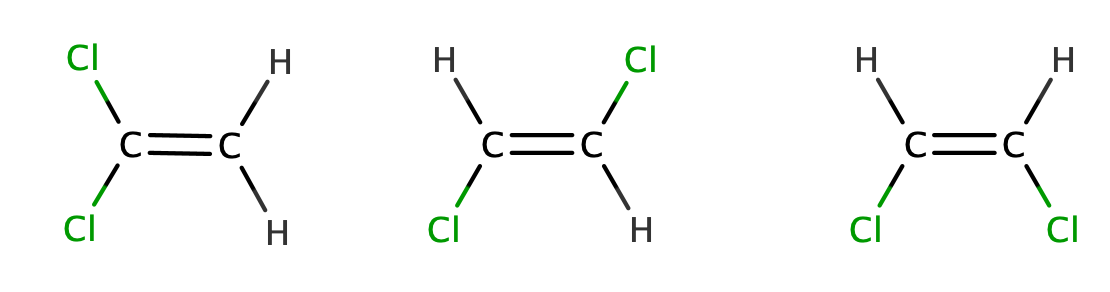
\includegraphics[width=\textwidth]{isomerer.png}
\end{center}
\caption{Strukturformlerne for de tre isomerer tegnet i MarvinSketch}
\label{fig:isomerer}
\end{figure}
\noindent \textbf{d.}
De fire isomere bromforbindelser kan ses i \cref{fig:bromforbindelser}.
De systematiske navne for de fire isomere bromforbindelser er henholdsvis 1,2-dibrom-1,1-dichlorethan, 1,2-dibrom-1,2-dichlorethan, 1,1-dibrom-1,2-dichlorethan og 1,1-dibrom-2,2-dichlorethan.
\begin{figure}[H]
\begin{center}
  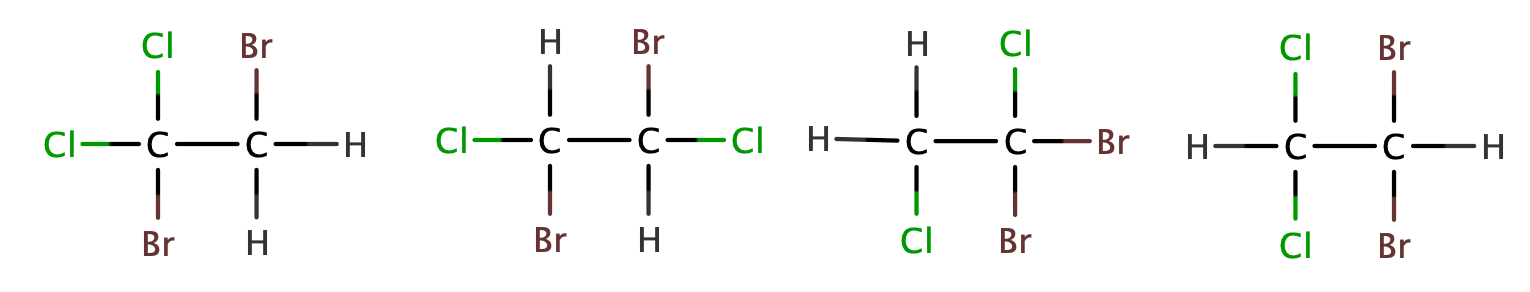
\includegraphics[width=\textwidth]{bromforbindelser.png}
\end{center}
\caption{Strukturformlerne for de fire isomere bromforbindelser tegnet i MarvinSketch}
\label{fig:bromforbindelser}
\end{figure}

\section*{Opgave 1.17}
\textbf{a.}
Afstemningen af reaktionsskemaet kan ses i \cref{fig:redox}.
\begin{figure}[H]
\begin{center}
  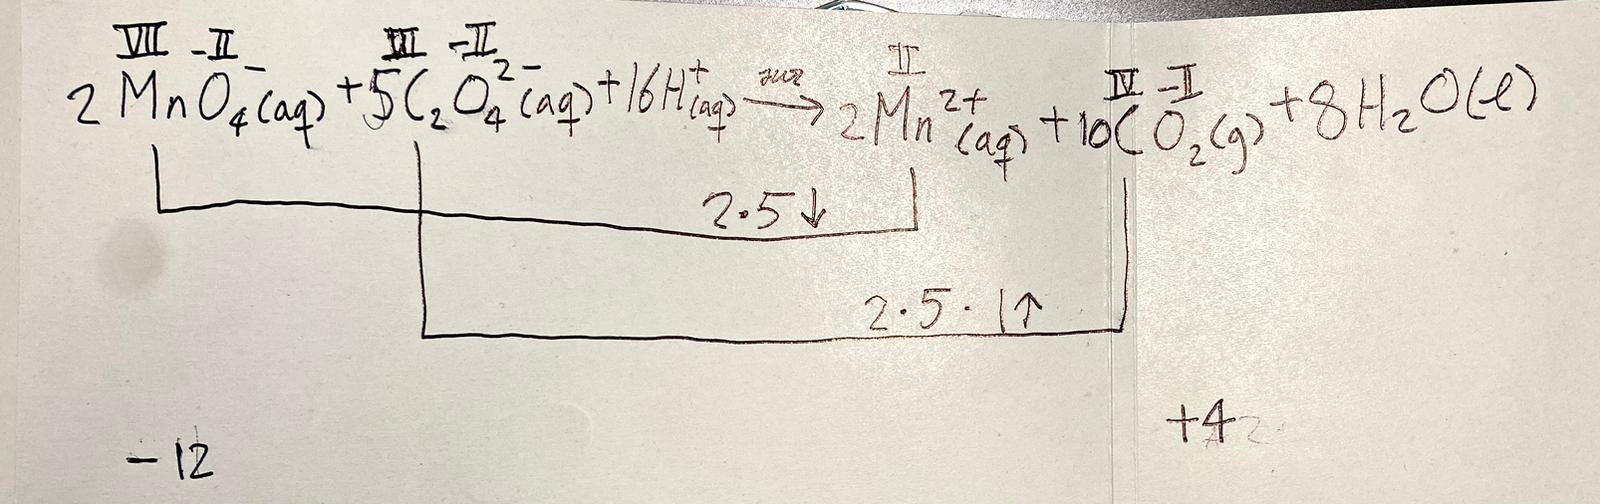
\includegraphics[width=\textwidth]{redox.jpeg}
\end{center}
\caption{Afstemning af reaktionsskemaet i hånden}
\label{fig:redox}
\end{figure}
\noindent\textbf{b.}
Fra \cref{fig:redox} ser vi, at reaktionsforholdet mellem \ce{MnO4-} og \ce{SO2} er 2:5.
Ved opløsningen af \ce{KMnO4} i vand er reaktionsforholdet mellem \ce{MnO4-} og \ce{KMnO4} da 1:1.
Vi kan nu regne stofmængden af \ce{SO2} ud i $200 \;\unit{mL} $ af vinen. 
\begin{equation*}
\begin{split}
  n(\ce{SO2}) &=\frac{5}{2} \cdot n(\ce{MnO4-} )\\ 
  &=\frac{5}{2} \cdot V(\ce{KMnO4}\text{-opl.})\cdot c(\ce{KMnO4} )\\ 
  &=\frac{5}{2} \cdot 9,10 \;\unit{mL} \cdot 0,0208 \;\unit{\textsc{m}}\\ 
  &=0,4732 \;\unit{mmol} 
\end{split}
\end{equation*}
\begin{note}
  Vi lader herunder $k(A) $ betegne den formelle stofmængdekoncentration af stoffet $A$ angivet i \unit{mg/L}.
\end{note}
Vi kan da nu regne den formelle stofmængdekoncentration af \ce{SO2} i vinen ud i \unit{mg/L}.
\begin{equation*}
\begin{split}
  k(\ce{SO2} )&=\frac{n(\ce{SO2} )\cdot M(\ce{SO2} )}{V}\\ 
  &=\frac{0,4732 \;\unit{mmol} \cdot 64,07 \;\unit{g/mol} }{0,200 \;\unit{L} }\\ 
  &\approx 152 \;\unit{mg/L} 
\end{split}
\end{equation*}
Altså er den formelle stofmængdekoncentration af \ce{SO2} i vinen $152 \;\unit{mg/L} $. \\[1ex]
\textbf{c.}
For den mængde natriumsulfit, der skal tilsættes per liter vin or at opnå et S-indhold af samme størrelse, må der gælde, at $\frac{c(\ce{SO2} )}{1 \;\unit{L} }=n(\ce{Na2SO3} )$.
Denne kan vi nu regne ud.
\begin{equation*}
\begin{split}
  n(\ce{Na2SO3} )&=0,4732 \;\unit{mmol} \cdot 5\\ 
  &=2,366 \;\unit{mmol} 
\end{split}
\end{equation*}
Vi regner nu massen denne mængde natriumsulfit.
\begin{equation*}
\begin{split}
  m(\ce{Na2SO3} )&=n(\ce{Na2SO3} ) \cdot M(\ce{Na2SO3} )\\
  &=2,366 \;\unit{mmol} \cdot 126,04 \;\unit{g/mol} \\ 
  &\approx 298 \;\unit{mg} 
\end{split}
\end{equation*}
Altså er massen af den mængde natriumsulfit, der skal tilsættes per liter vin for at opnå et S-indhold af samme størrelse som i den undersøgte vin $298 \;\unit{mg} $.
Ved at kigge på EU-listen kan man se, at den maksimale mængde er $200 \;\unit{mg/L} $.
Altså er vores udregnede mængde natriumsulfit større end værdien givet ved EU-listen.

\section*{Opgave 2.20}
\textbf{a.}
I \cref{fig:reak} ses, hvorledes 2-chlor-3-methylhexan kan dannes ud fra 3-methylhex-1-en.
Læg mærke til, at 2-chlor-3-methylhexan er det primære produkt, da chlor-atomet især vil binde sig til det sekundære \ce{C}-atom frem for det primære.
\begin{figure}[H]
\begin{center}
  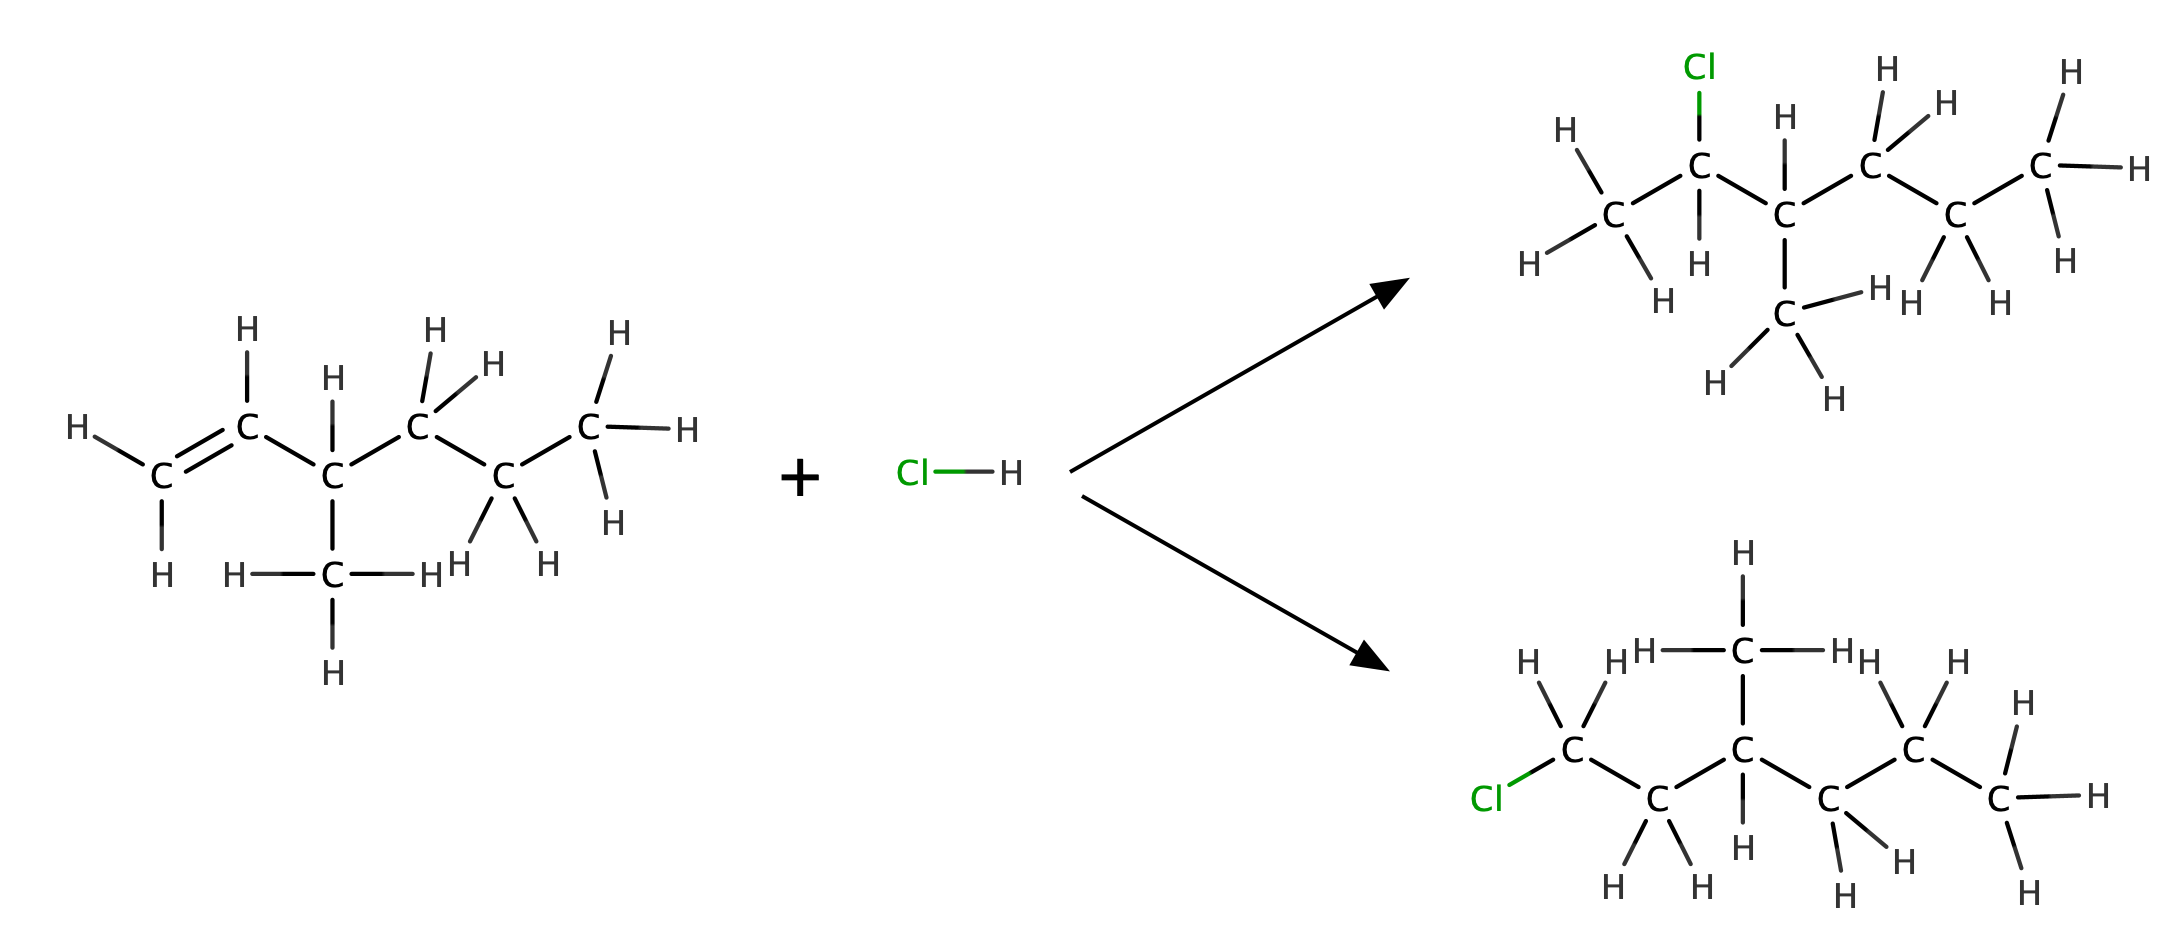
\includegraphics[width=\textwidth]{reak.png}
\end{center}
\caption{2-chlor-3-methylhexan dannet ud fra 3-methylhex-1-en}
\label{fig:reak}
\end{figure}
\noindent\textbf{b.}
Der er 1 assymetrisk \ce{C}-atom i 3-methylhex-1-en, og der er ingen geometriske isomerer eller diastereomerer.
Altså er der 2 stereoisomere former for 3-methylhex-1-en.

For 2-chlor-3-methylhexan er der ingen geometriske isomerer.
Der er dog to assymetriske \ce{C}-atomer.
Altså er der $2^2=4$ stereoisomere former for 2-chlor-3-methylhexan.
\end{document}
